% =============================================================================
% File      : ex_doc_2-32.tex -- example 2.32
% Author    : Jürgen Hackl <hackl.j@gmx.at>
% Creation  : 2019-08-14
% Time-stamp: <Wed 2019-08-14 17:07 juergen>
%
% Copyright (c) 2019 Jürgen Hackl <hackl.j@gmx.at>
% =============================================================================
\documentclass{standalone}
\usepackage{../../tikz-network}
\begin{document}
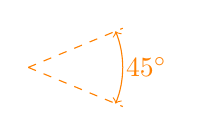
\begin{tikzpicture}
  \Vertex{A}
  \Edge[loopshape=45](A)(A)
  \draw[orange,dashed](0,0) -- (-22.5:13mm)(0,0)--(22.5:13mm);
  \draw[orange,->] (1.2,0) arc (0:22.5:12mm);
  \draw[orange,->] (1.2,0) arc (0:-22.5:12mm);
  \node[orange] (x) at (1.5,0) {$45^\circ$};
\end{tikzpicture}
\end{document}
% =============================================================================
% eof

%%% Local Variables:
%%% mode: latex
%%% TeX-master: t
%%% End:
